\documentclass[a5paper,10pt,oneside,landscape]{article}

\usepackage[swedish]{babel}
\usepackage[T1]{fontenc}
\usepackage[latin1]{inputenc} % Denna m�ste �ndras till r�tt teckenkodning f�r er

\usepackage{graphicx}
\usepackage{url}
%\usepackage{ifthen}
\usepackage[a5paper,margin=1.5cm,noheadfoot]{geometry}

\usepackage{listings}
\lstset{language=Java,numbers=left,frame=L,floatplacement=hbtp}
\def \lstlistingname {Kodexempel}

\usepackage{ifpdf}
\ifpdf
	\usepackage[hidelinks]{hyperref}
\else
	\usepackage{url}
\fi
\newcommand{\avsnitt}[1]{\newpage\section*{#1}}

\begin{document}

%%%%%%%%%%%%% Framsidan %%%%%%%%%%%%%%

\title{Projektnamn}
\author{Adam Alfa\\adal1234 \and Beatrice Beta\\bebe5678 \and Caesar Gamma\\caga9012 \and Diana Delta\\dide3456}
\maketitle

%%%%%%%%%%%%% Rapportens delar %%%%%%%%%%%%%%%

\avsnitt{Introduktion}

En kort introduction till projektet d�r ni ocks� listar de verktyg ni anv�nt. Om ert versionshanteringssystem g�r att komma �t ska adressen dit finnas med, annars ska det finnas en l�nk fr�n vilken man kan ladda hem k�llkoden.

-----------------

\avsnitt{Slutlig design}
Vi valde att dela upp v�rat projekt p� ett s�dant sett att det finns ett separat paket som heter \emph{cards} vilket �r t�nkt som ett allm�nt kortspels-paket med kort, kortlekar, spelare, h�nder osv och sedan ett paket, \emph{texasholdem}, som �r mer specifikt inriktat p� kortspelet Texas Holdem. I det senare ligger ocks� s�dant som mer styr spelregler och spelmekaniken.

Nedan �r ett klassdiagram �ver hela v�rt projekt:\\
\DeclareGraphicsExtensions{.png}
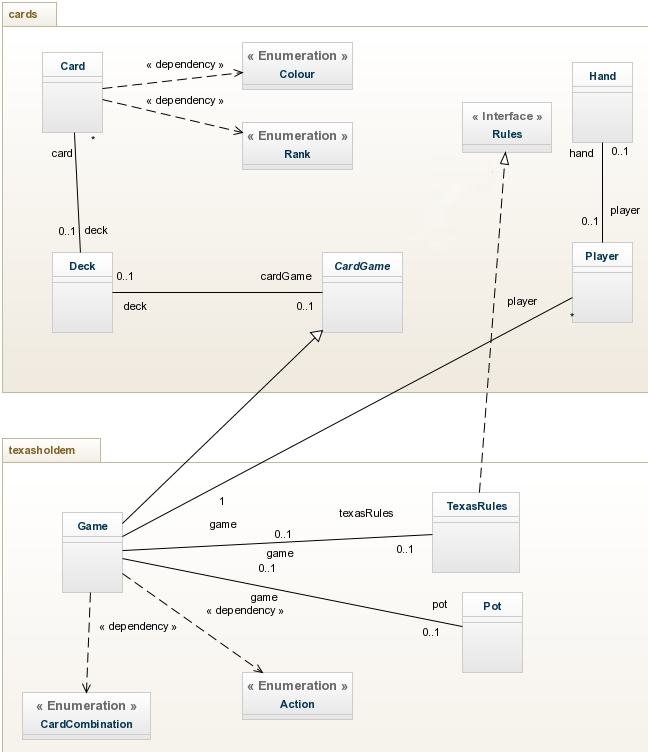
\includegraphics[natwidth=848, natheight=958, scale=0.73, angle=0, trim = 0mm 0mm 42mm 16mm]{bilder/diagram/klassdiagram-2014-10-28}

Samt n�gra mer detaljerade diagram �ver projektet;

\DeclareGraphicsExtensions{.png}
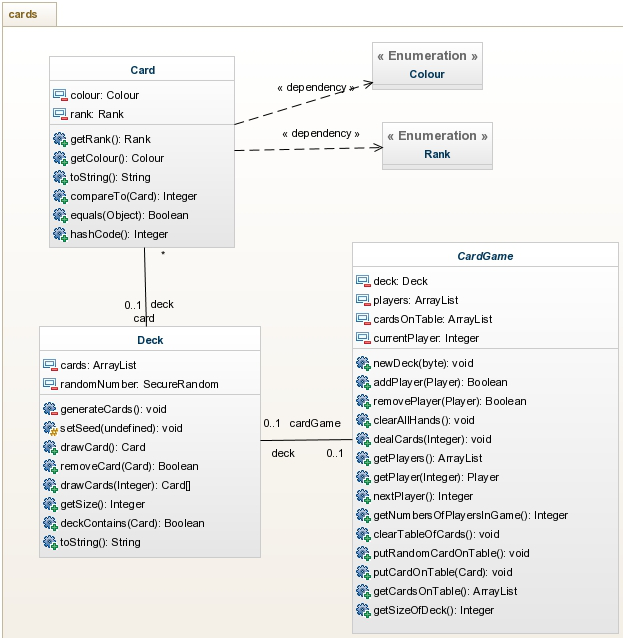
\includegraphics[natwidth=623, natheight=638, scale=0.91, angle=0, trim = 0mm 0mm 0mm 26mm]{bilder/diagram/card1}

\DeclareGraphicsExtensions{.png}
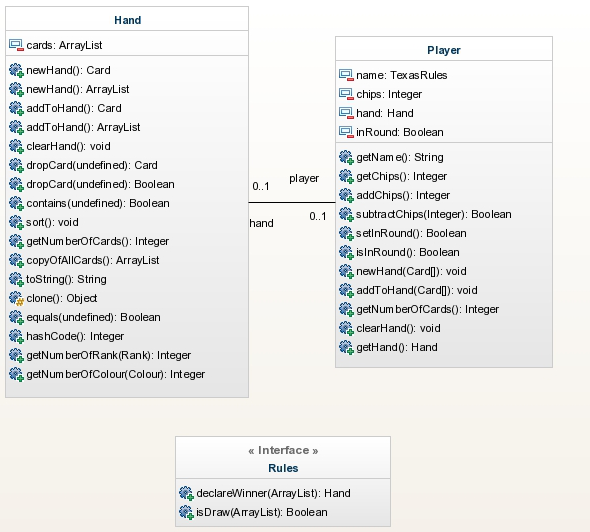
\includegraphics[natwidth=590, natheight=532, scale=0.95, angle=0, trim = 0mm 0mm 0mm 5mm]{bilder/diagram/card2}

\DeclareGraphicsExtensions{.png}
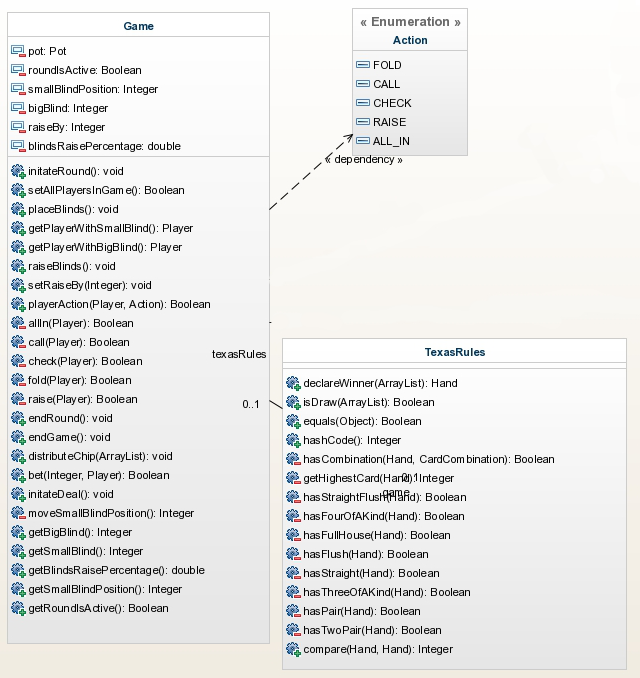
\includegraphics[natwidth=640, natheight=678, scale=0.84, angle=0, trim = 0mm 0mm 0mm 19mm]{bilder/diagram/texas1}

\DeclareGraphicsExtensions{.png}
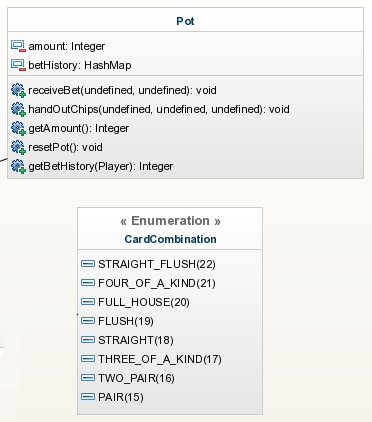
\includegraphics[natwidth=372, natheight=422, scale=1, angle=0, trim = 0mm 0mm 0mm 0mm]{bilder/diagram/texas2}

\avsnitt{Testdriven utveckling -- process}

Alla fyra har till�mpat testdriven utveckling under st�rre delar av projektets g�ng.
Till en b�rjan var vi h�rda p� att anv�nda testdriven utveckling men desto l�ngre in i projektet vi kom s� sl�ppte vi p� det f�r att f� in alla funktioner i programmet.
�ven om vi inte var lika h�rda i slutet p� att till�mpa testdriven utveckling s� �vergav vi �nd� inte det helt d� vi k�nde att det var ett v�ldigt anv�nbart verktyg. I den senare delen av projektet kom dock testfallen - tyv�rr - oftast att skrivas efter att koden som skulle testas redan hade skrivits.

Nedan kommer 4 olika exempel p� testfall som skrivits av alla personer i projektet och den kom som togs fram med hj�lp av testfallen:

Elliot : PotTest\\
\begin{lstlisting}
@Test
public void betSizeTestFromEmptyPot(){
	Pot emptyPot = new Pot();
	emptyPot.receiveBet(300,player1);
	assertEquals(300, emptyPot.getAmount());
}

@Test
public void betSizeTestFromPositiveSize() {
	Pot positivePot = new Pot(1);
	positivePot.receiveBet(300,player1);
	assertEquals(301, positivePot.getAmount());
}
\end{lstlisting}

Elliot : Pot.receiveBet()\\
\begin{lstlisting}
public void receiveBet(int bet, Player player) {
	if (bet < 1)
		throw new IllegalArgumentException(
				"The Bet has to be larger than 0");
	else {
		amount += bet;
		betHistory.put(player, this.getBetHistory(player) + bet);
	}
}
\end{lstlisting}

Rasmus : PotTest\\
\begin{lstlisting}
@Test(expected = IllegalArgumentException.class)
	public void testForInvalidSize() {
		Pot invalidPot = new Pot(-1);
		assertEquals(-1, invalidPot.getAmount());
	}

@Test
	public void testPotSizeIfPositiveInt() {
		Pot pot = new Pot(500);
		assertEquals(500, pot.getAmount());
	}
\end{lstlisting}

Rasmus : Pot.Pot()\\
\begin{lstlisting}
public Pot(int amount) {
		if (amount < 0)
			throw new IllegalArgumentException(
					"The Pot has to be at least 0");
		this.amount = amount;
	}
\end{lstlisting}

Emil : GameTest\\
\begin{lstlisting}
@Test
public void addingOnePlayerTest(){
	Game newGame = new Game(4, 0.3, kalle);
	assertTrue(newGame.getPlayers().contains(kalle));
}

@Test
public void addingPlayersTest(){
	Game newGame = new Game(4, 0.3, kalle, pelle);
	assertTrue(newGame.getPlayers().contains(kalle));
	assertTrue(newGame.getPlayers().contains(pelle));
}
\end{lstlisting}

Emil : Game.Game()\\
\begin{lstlisting}
public Game(int bigBlind, double blindsRaisePercentage, Player... players) {
		this(players);
		if (bigBlind < 1)
			throw new IllegalArgumentException(
					"Error: parameter bigBlind is less than 1.");
		if (blindsRaisePercentage < 0)
			throw new IllegalArgumentException(
					"Error: parameter blindsRaisePercentage is less than 0.");
		this.bigBlind = bigBlind;
		this.blindsRaisePercentage = blindsRaisePercentage;
	}
\end{lstlisting}

Anton : CardTest\\
\begin{lstlisting}
@Test
public void testEqualsValid(){
        Card card1 = new Card(Colour.HEARTS, Rank.QUEEN);
        Card card2 = new Card(Colour.HEARTS, Rank.QUEEN);
        assertTrue(card1.equals(card2));
}

@Test
public void testEqualsInvalid(){
        Card card1 = new Card(Colour.HEARTS, Rank.QUEEN);
        Card card2 = new Card(Colour.HEARTS, Rank.ACE);
        assertFalse(card1.equals(card2));
        card2 = new Card(Colour.CLUBS, Rank.QUEEN);
        assertFalse(card1.equals(card2));
        card2 = null;
        assertFalse(card1.equals(card2));
        assertFalse(card1.equals("A string"));
}
\end{lstlisting}

Anton : Card.equals()\\
\begin{lstlisting}
@Override
public boolean equals(Object object){
        if(object == null)
                return false;
        if(!object.getClass().equals(this.getClass()))
                return false;
        Card other = (Card) object;
        return (this.colour.equals(other.colour) && this.rank.equals(other.rank));
}
\end{lstlisting}

\avsnitt{Testdriven utveckling -- erfarenheter}

Vi har arbetat med testdriven utveckling n�stan helt och h�llet genom projektet vilket har gett oss en m�ngd erfarenheter av hur bra/d�ligt det kan fungera.
Till en b�rjan k�ndes det v�ldigt �verfl�digt och framtvingat d� man arbetade med simpla metoder,
klasser och konstruktioner som k�ndes sj�lvklara hur man skulle skriva och som alltid fungerade direkt.
Desto mer vi arbetade och kom in i sv�rare metoder och konstruktioner s� b�rjade testdriven utveckling k�nnas mer och mer anv�ndbart och mot slutet i projektet,
speciellt n�r vi arbetade med klasses TexasRules, s� k�ndes det n�stan som att det hade varit om�jligt att genomf�ra den delen utan testdriven utveckling och testfall.
Eftersom man i klassen TexasRules beh�vde testa v�ldigt specifika fall, som t ex att r�tt person vinner om b�da har stege men en av personerna har h�gre kort,
s� gjorde testfall att man enkelt kunde s�tta upp ett eller flera komplexa fall som endast g�tt igenom om koden �r korrekt skriven.
Detta skulle vara v�ldigt sv�rt att testa utan testfall.

Testdriven utveckling ledde ocks� till att vi snabbt uppt�ckte fel som introducerats i koden.
Detta eftersom man kunde se om ett testfall g�tt igenom tidigare antingen i commit-kommentarerna eller f�r att man sj�lv k�rt dem tidigare och
d� ocks� se om man kan ha introducerat n�got fel i en specifik del av koden. Lyckades man d� inte se vilket fel man introducerat
s� gick det alltid att titta p� versionen som commitats t ex med kommentaren \emph{testfall X g�r nu igenom} och se hur koden s�g ut i det tillf�llet.

En ytterliggare positiv effekt av testdriven utveckling som vi inte t�nkt p� i f�rhand �r att den g�r koden mycket mer l�ttf�rst�elig
f�r de man arbetar med d� man kan se hur koden �r t�nkt att fungera �ven om den inte i nuvarande l�ge fungerar. Detta leder till att man enkelt kan ta �ver metoder
och skriva klart dem �ven om det inte var man sj�lv som b�rjade skriva p� den. �ven om man har dokumentation om ungef�r vad metoden ska g�ra,
s� ger testfallen mycket med information om exakt hur metoden ska bete sig och vilket resultat som f�rv�ntas.

Vi har f�rst�s ocks� f�tt uppleva n�gra utav baksidorna med testdriven utveckling. Det �r tidskr�vande,
speciellt att skriva bra tester som ger god t�ckningsgrad och t�cker alla ekvivalensklasser.
Det kr�vs god disciplin f�r att inte slarva och b�rja �verg� i ad-hoc-testning, speciellt under tidspress,
n�got som vi kanske inte kan s�ga att vi alltid lyckats med. Det �r inte heller alla g�nger som vi varit helt �verens om hur vi ska prioritera testbarhet kontra inkapsling.
Oftast har vi lyckats finna n�gon kompromiss d�r t.ex. privata metoder har varit testbara via publika metoder d�r den privata anropas.

\avsnitt{Ekvivalensklassuppdelning -- subtractChips}

En kort presentation av vad ni valt ut f�r att till�mpa ekvivalensklassuppdelning p�. Ni ska kort motivera valet, och ge tillr�ckligt med information f�r att det ska g� att bed�ma er. Detta avsnitt och de tre f�jande (till och med testmatrisen) ska finnas f�r samtliga delar ni till�mpat ekvivalensklassuppdelning p�.
D� vi inte hittade n�gra sj�lvklara metoder att k�ra ekvivalensklassuppdelning vid en f�rsta anblick s� valde vi att g�ra det p� n�gra klasser som anv�nds relativt ofta och/eller som �r v�ldigt viktiga att ingenting f�r g� fel i. subtractChips �r en metod
som �r v�ldigt viktigt att den fungerar som den ska och returnerar r�tt v�rde vid r�tt tillf�lle d� det annars kan leda till att en person som ej har r�d att betala en viss summa till potten �nd� kan f� forts�tta den rundan. Vi valde d�rf�r att genomf�ra ekvivalensklassuppdelning
p� denna metod f�r att se till att vi inte missat n�got �ven fast det inte resulterade i j�tte m�nga ekvivalensklasser.

-----------------

\avsnitt{Ekvivalensklasser -- subtractChips}

Samtliga ekvivalensklasser f�r denna del presenterade p� ett tydligt s�tt.\\
-----------------\\

public boolean subtractChips(int bet)

\begin{table}[h]
\begin{tabular}{|l|l|l|l|l|l|}
\hline
Ekvivalensklass \cellcolor{red!15} & \multicolumn{2}{|l|}{\textbf{Invalida interval} \cellcolor{red!15}} &
Ekvivalensklass \cellcolor{green!15} & \multicolumn{2}{|l|}{\textbf{Valida interval} \cellcolor{green!15}} \\ \hline
\cellcolor{red!15} a	& int bet \cellcolor{red!15}		& $<=0$ \cellcolor{red!15}		& \cellcolor{green!15}	c						& int bet \cellcolor{green!15}					& $0<bet<=chips$ \cellcolor{green!15}	\\ \hline
\cellcolor{red!15} b	& int bet	\cellcolor{red!15}		& $>chips$ \cellcolor{red!15}	& \cellcolor{green!15}							& \cellcolor{green!15}							& \cellcolor{green!15}					\\ \hline
\end{tabular}
\end{table}



\avsnitt{Testfall -- subtractChips}

Testfallen som ni f�tt fram fr�n ekvivalensklasserna. Observera att vi inte vill ha n�gon kod h�r, utan bara en tydlig presentation av testfallen i n�gon l�mplig tabellform.
\begin{table}[h]
\begin{tabular}{|l|l|l|l|}
\hline
id & Namn &Input(int bet) & Resultat \\ \hline
\rowcolor{green!15}
1  & addToPotTestSuccess()	& 1              & true   \\ \hline
\rowcolor{green!15}
2  & addToPotTestSuccess()	& chips          & true   \\ \hline
\rowcolor{red!15}
3  & add0ChipsToPotTest()	& 0              & false  \\ \hline
\rowcolor{red!15}
4  & addToPotTestFail()	& chips+1        & false	 \\ \hline
\end{tabular}
\end{table}

\avsnitt{Testmatris -- subtractChips}

En testmatris som visar sambandet mellan ekvivalensklasserna och testfallen f�r denna del.


\begin{table}[h]
\begin{tabular}{|l|l|l|l|}
\hline
  & a & b & c \\ \hline
1 &   &   & x \\ \hline
2 &   &   & x \\ \hline
3 & x &   &   \\ \hline
4 &   & x &		\\ \hline
\end{tabular}
\end{table}

\avsnitt{Ekvivalensklassuppdelning - Game-konstruktor}

En kort presentation av vad ni valt ut f�r att till�mpa ekvivalensklassuppdelning p�. Ni ska kort motivera valet, och ge tillr�ckligt med information f�r att det ska g� att bed�ma er. Detta avsnitt och de tre f�jande (till och med testmatrisen) ska finnas f�r samtliga delar ni till�mpat ekvivalensklassuppdelning p�.\\
----------------------------------------\\
Vi valde att g�ra en ekvivalensklassuppdellning p� Game-konstruktorn d� den tar emot relativt m�nga parametrar, iallfall om man j�mf�r med resten av projektet, och l�per d�rf�r en st�rre risk att f� olika slags fel. Den �r ocks� en v�ldigt viktig del av hela biblioteket
d� det �r objekt av denna klass som skapas n�r man vill starta ett Texas Holdem-spel vilket gjorde att den k�ndes som en sj�lvklar metod att till�mpa ekvivalensklassuppdelning p�.

\avsnitt{Ekvivalensklasser -- Game-konstruktor }

Samtliga ekvivalensklasser f�r denna del presenterade p� ett tydligt s�tt.

\begin{table}[h]
\begin{tabular}{|>{\columncolor{green!15}}l|>{\columncolor{green!15}}l|>{\columncolor{green!15}}l|} \hline
Ekvivalensklass                         & \multicolumn{2}{l|}{\cellcolor{green!15}\textbf{Valida intervall}}\\ \hline
a                                       & int bigBlind                                         & \textgreater0 \\ \hline
b                                       & double blindsRaisePercentage                         & \textgreater=0 \\ \hline
c                                       & Player... players                                    & >0 \\ \hline
d                                       & Player... players                                    & 0 \\ \hline
\cellcolor{red!15}Ekvivalensklass & \multicolumn{2}{l|}{\cellcolor{red!15}\textbf{Invalida intervall}} \\ \hline
\cellcolor{red!15}e               & \cellcolor{red!15}int bigBlind                 & \cellcolor{red!15}\textless=0 \\ \hline
\cellcolor{red!15}f               & \cellcolor{red!15}double blindsRaisePercentage & \cellcolor{red!15}\textless0 \\ \hline
\cellcolor{red!15}g               & \cellcolor{red!15}Player... players            & \cellcolor{red!15}null \\ \hline
\end{tabular}
\end{table}

\avsnitt{Testfall -- Game-konstruktor }

\begin{table}[h]
\begin{tabular}{|l|l|l|l|l|l|}
\hline
id & Namn                                       & \textit{bigBlind} & \textit{blindsRaisePercentage} & \textit{players} & Resultat                 \\ \hline
\rowcolor{green!15}
1  & assertBlindsAndPlayersInNewGameTest()      & 4                 & 0.3                            & 2                & \checkmark               \\ \hline
\rowcolor{green!15}
2  & addingNoPlayerTest()                       & 4                 & 0.3                            & 0                & \checkmark               \\ \hline
\rowcolor{red!15}
3  & addingNegativeBigBlindTest()               & -4                & 0.3                            & 1                & IllegalArgumentException \\ \hline
\rowcolor{red!15}
4  & addingNegativeBlindsRaiserPercentageTest() & 4                 & -0.2                           & 1                & IllegalArgumentException \\ \hline
\rowcolor{red!15}
5  & nullPlayerConstructorTest()                & 2					& 0.5                            & null             & NullPointerException \\ \hline
\end{tabular}
\end{table}

\avsnitt{Testmatris -- Game-konstruktor }

\begin{table}[h]
\begin{tabular}{|c|c|c|c|c|c|c|c|}
\hline
  & a & b & c & d & e & f & g \\ \hline
1 & x & x & x &   &   &   &   \\ \hline
2 & x & x &   & x &   &   &   \\ \hline
3 &   &   &   &   & x &   &   \\ \hline
4 &   &   &   &   &   & x &   \\ \hline
5 &   &   &   &   &   &   & x \\ \hline
\end{tabular}
\end{table}


\avsnitt{Tillst�ndsbaserad testning}

En kort presentation av vad ni valt ut f�r att till�mpa tillst�ndsbaserad testning p� och 
vilket t�ckningskriterium ni valt att anv�nda er av. 
Ni ska kort motivera valen, och ge tillr�ckligt med information f�r att det ska g� att bed�ma er. 
Gl�m inte att ta med sj�lva modellen.

Vi valde att till�mpa tillst�ndsbaserad testning p� v�r Player-klass eftersom den hanterar de tillst�nd som en spelare kommer att f�rflyttas emellan under hela spelets g�ng.
Statement coverage �r det t�ckningskriterium som vi valde att anv�nda oss av eftersom det kollar varje programsats genom programmet och kan se till att det har en h�g t�ckningsgad. 
H�r velade vi lite mellan om vi skulle statement och branch coverage, vi ans�g att det inte skulle spela n�gon st�rre roll och 
vi ville se att t�ckningsgraden h�ller en s� pass h�g grad som m�jligt i funktionerna och best�mde oss f�r att anv�nda statement coverage.
Modellen som vi designade visar p� hur klassen hanterar en spelare i v�rt system och vilka tillst�nd denne spelare kan befinna sig i.


\avsnitt{Testfall f�r tillst�ndsbaserad testning}

Testfallen som ni f�tt fram fr�n tillst�ndsmaskinen. Observera att vi inte vill ha n�gon kod h�r, 
utan bara en tydlig presentation av testfallen i n�gon l�mplig tabellform. 
Det ska enkelt g� att mappa testfallen till tillst�ndsmaskinen.

Testfallen vi skrev gjordes efter det att modellen hade gjorts och d�rmed till�mpade vi inte testdriven utveckling under denna del av projektet
d� vi inte k�ndes oss helt s�kra p� hur mycket vi skulle ha med i modellen fr�n b�rjan.
Under tiden d� modellen designades s� diskuterades det runt andra m�jliga tillst�nd som man komma till eftersom koden runt dessa tillst�nd vi redan hade inte var kompletta, 
vi best�mde oss f�r att g�ra klart modellen efter det vi hade i koden just d� och designa testfallen efter tillst�nden vi redan hade. 

testfallen i n�gon l�mplig tabellform
\avsnitt{Kodkritiksystem}


En presentation av de problem som hittats med hj�lp av verktyg f�r statisk analys och en diskussion av dem enligt anvisningarna. Det r�cker allts� inte med att bara lista problemen, ni m�ste f�rh�lla er till dem ocks�. T�nk ocks� p� att ni ska g�ra detta b�de p� koden som den s�g ut f�re granskningen och p� koden efter att ni r�ttat det som kommit fram under granskningen.

-----------------

Vi k�rde FindBugs vid ett flertal tillf�llen under utvecklingen med olika resultat men den slutsatsen vi �nd� kunde dra av detta var att FindBugs var en av de minst anv�ndbara verktygen vi testat oss p�,
n�r den anv�ndes f�r f�rsta g�ngen precis innan den f�rsta granskningen s� hittade den inte ett enda fel, �ven n�r k�nsligheten drogs upp p� max och vi bad den rapportera allt den m�jligen kunde hitta.
Det fanns dock inga st�rre fel vid denna punkt men vi hittade �nd� r�tt mycket saker som vi beh�vde �ndra n�r vi k�rde v�r formella granskning som FindBugs ej hade hittat. M�nga av de felen vi hittade
hade dock med namngivning och liknande att g�ra vilket �r sv�rare f�r ett program att hitta. Vi k�rde ocks� FindBugs efter vi gjort korrigeringar efter granskningen men hittade d� heller inga fel.
Vi k�rde d�remot FindBugs mot slutet av projektet ocks� och d� hittade den faktist n�gra intressanta fel som hj�lpte oss:
/*s�tt in fel som hittas nu i koden*/

\avsnitt{Statiska m�tt}

En presentation och diskussion kring ett antal l�mpliga statiska m�tt p� koden. Att vi inte specificerar exakt vilka m�tt som ska tas upp beror p� att olika verktyg har olika upps�ttningar, men vi f�rv�ntar oss fler och mer intressanta m�tt �n bara rena storleksm�tt som LOC, \#klasser, \#metoder, etc. �ven h�r �r det viktigt att f�rh�llas sig till m�tten, inte bara lista dem.

\textbf{Number of Classes}: 8 (exklusive testfall, interface och enums)
\begin{enumerate}
	\item cards: 5
	\item texasholdem: 3
\end{enumerate}

\textbf{Total Lines of Code}: 2014
\begin{enumerate}
	\item testfall: 1140 (56,6\%)
	\item texasholdem: 476  (23,6\%)
	\item cards: 398 (19,7\%)
\end{enumerate}

Det som kan vara intressant med resultaten f�r \emph{Number of Classes} och \emph{Total Lines of Code} �r det faktum att paketet texasholdem har f�rre klasser �n cards, men fler antal rader kod. Man b�r kanske fundera p� varf�r det har blivit s�, och fr�ga sig om det verkligen �r bra. Detta �r n�got som i sin tur st�r i korrelation till de metrics som f�ljer.

\textbf{Lack of Cohesion (mean)}:  0,403
\begin{enumerate}
	\item Game: 0,806
	\item Player: 0,795
	\item CardGame: 0,717
\end{enumerate}

Kanske inte helt ov�ntat s� �r den st�rsta klassen, Game, den som har h�gst avsaknad av coheshion. Intresasnt �r att i ett tidigare skede s� var Game och CardGame en och samma klass, och trots denna uppdelning s� har b�da dessa vuxit p� ett s�tt som kanske inte �r �nksv�rt. B�de Game och CardGame b�rjar f� lite \emph{God-klass}-tendenser och b�r ses �ver.  Vi har sagt att om vi v�ljer att forts�tta att utveckla v�rt bibliotek s� kommer en ytterliggare uppdelning av n�gon (eller alla) av de tre klasserna vara aktuellt. Player sticker ut lite som �r en ganska liten klass j�mf�rt med de andra tv� (ca 60 LoC j�mf�rt med 230 respektive 110) men trots det s� har den r�tt stor avsaknad av cohesion. De flesta av klassens metoder arbetar antingen p� variablen \emph{chips} eller objektet \emph{hand}, men ingen av klassens metoder arbetar p� b�da dessa. Resultat �r med andra ord inte s� f�rv�nande.

Eftersom att hantering av chips inte �r en funktion som �r generell f�r alla kortspel, s� b�r vi kanske �verv�ga att avl�gsna chips-hanteringen fr�n den generella klassen Player och l�gga in i en separat klass, m�jligen en subklass.\\

\textbf{MacCabe Cyclomatic Complexity (mean)}: 1,632
\begin{enumerate}
	\item Pot:handOutChips() - 9
	\item TexasRules:hasCombination() - 9
	\item Game:placeBlinds() - 7
	\item Game:playerAction() - 7
\end{enumerate}

Den relativt sett h�ga komplexiteten p� n�gra av de metoder som finns ger kanske en fingervisning om att det finns utrymme f�r f�rb�ttring. Metoderna handOutChips och placeBlinds skulle f�rmodligen kunna refaktoriseras och delas upp i flera mindre metoder f�r att minska komplexiteten n�got, �ven om komplexiteten i sig g�r det sv�rare. Metoderna hasCombination och playerAction har lika h�g komplexitet som de nyss n�mnda, men detta fr�mst till f�ljd av att de har switch-satser, varf�r de kan vara en �n st�rre utmaning att dela upp dem i flera mindre metoder.\\


\textbf{Number of Parameters (mean)}: 0,667
\begin{enumerate}
	\item Pot:handOutChips(Player player, int chipsWon, int playersWon) - 3
	\item Game:Game(int bigBlind, double blindsRaisePercentage, Player... players) - 3
\end{enumerate}

Vi har �verlag lyckats h�lla nere antalet parametrar f�r metoderna i v�rt bibliotek. Kontruktorn ovan beh�ver dessutom bara tv� av de tre argumenten d� den sista �r en varargs som inte �r obligatorisk.

\textbf{Method Lines of Code (mean)}: 4.313
\begin{enumerate}
	\item Pot:handOutChips() - 34
	\item Game:distributeChip() - 22
	\item Game:placeBlinds() - 14
\end{enumerate}

Som man kanske hade kunnat gissa s� kan man se ett samband mellan \emph{MacCabe Cyclomatic Complexity} och \emph{Method Lines of Code} d�r en mer komplex metod kan utg�ra ett motst�nd f�r att bryta upp den i flera mindre metoder.

Dessa statiska m�tt �r var och f�r sig, av ganska begr�nsad nytta, men tillsammans ger de en ganska god bild av vilka f�rb�ttringar som k�ras p� projektet som helhet och enskilda klasser och metoder.


\textbf{Pizza metric index}: 1\\
Vi har inte r�d att �ta mer pizza.

\avsnitt{T�ckningsgrad}

En �versikt �ver vilken t�ckningsgrad era testfall uppn�tt. Denna kan antagligen tas rakt av fr�n verktyget ni anv�nt f�r att m�ta den. Om ni inte uppn�tt fullst�ndig t�ckning s� ska detta f�rklaras och motiveras.

-------

Vi har n�rmast 100\% t�ckningsgrad. Det finns tv� klasser som inte riktigt n�r hela v�gen. I det ena fallet handlar det om klassen Deck som har en metod setSeed som matar ett SecureRandom-objekt med ny data f�r seeden. Metoden �r protected och anropas aldrig i dagsl�get av n�gon annan metod i paketet d� vi �r os�kra p� om vi faktiskt beh�ver den eller inte. Det kan faktiskt vara s� att vi kommer ta bort metoden, men fram till dess att vi �r helt s�kra p� att det �r r�tt beslut f�r den ligga kvar.

Den andra klassen som inte har 100\% t�ckningsgrad �r TexasRules. Det �r helt enkelt f�r att vi har kommit fram till att stora delar av koden m�ste skrivas om, och vi ser ingen po�ng med att f�rs�ka f� full t�ckning f�r kod som vi kommer ta bort.

\DeclareGraphicsExtensions{.png}
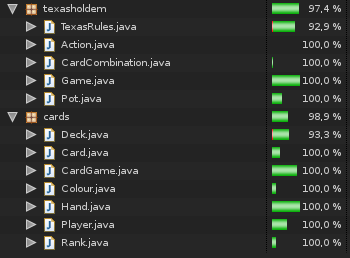
\includegraphics[natwidth=350, natheight=258, scale=0.9, angle=0, trim = 0mm 0mm 0mm 0mm, clip]{bilder/coverage}\\


\avsnitt{Profiler}

En kort presentation av hur ni g�tt tillv�ga f�r att testa koden med en profiler och vilka resultat ni fick fram.

\avsnitt{Byggscript}

Byggscriptets f�rsta (seri�sa) version, och den slutliga.

I den f�rsta versionen av byggscriptet var ambitionen fr�mst att det skulle g�ra ungef�r samma sak som den standard-byggscripten som eclipse skapar f�r ett projekt. Med andra ord, kompilera alla klasser och dess beroenden. Det gick ganska bra fram till dess att testfallen inkluderades, d� det kr�vdes externa bibliotek (JUnit) f�r att kompilera dessa. S� sm�ningom fick vi �ven det att fungera.

 \lstset{
	language=XML,
	basicstyle=\ttfamily\scriptsize,
	keywordstyle=\color{blue}\ttfamily,
	stringstyle=\color{red}\ttfamily,
	showspaces=false,
	breaklines=true
 }

\begin{lstlisting}[float,caption={build.xml, f�rsta versionen},label=lst]
<?xml version="1.0"?>
<project name="texas" default="buildTest" basedir=".">
<property name="build.dir" location="bin" />
<property name="srcCards.dir" value="src/cards" />
<property name="srcTexasHoldem.dir" value="src/texasholdem" />
<property name="srcTest.dir" value="test" />

<property name="test.report.dir" location="testreports" />

<path id="junit.class.path">
	<pathelement location="${eclipse}/plugins/org.junit*/*junit.jar" />
	<pathelement location="/home/anton/dokument/eclipse/plugins/org.junit_4.11.0.v201303080030/junit.jar" />
	<pathelement location="${eclipse}/plugins/*org.hamcrest.*.jar" />
	<pathelement location="${build.dir}" />
</path>

<target name="buildCards" description="Build package cards">
	<mkdir dir="${build.dir}" />
	<javac includeantruntime="false" destdir="${build.dir}" source="1.7" target="1.7">
		<src path="${srcCards.dir}"/>
	</javac>
</target>

<target name="buildTexas" description="Build package texas" depends="buildCards">
	<javac includeantruntime="false" destdir="${build.dir}" source="1.7" target="1.7">
		<src path="${srcTexasHoldem.dir}"/>
	</javac>
</target>

<target name="buildTest" description="Build test cases" depends="buildTexas">
	<mkdir dir="${build.dir}/test" />
	<javac includeantruntime="false" destdir="${build.dir}/test" source="1.7" target="1.7">
		<classpath refid="junit.class.path" />
		<src path="${srcTest.dir}"/>
	</javac>
</target>
</project>
\end{lstlisting}

I den f�rdiga versionen s� k�rs �ven testfallen, och om desa g�r igenom skapas �ven en jar-fil f�r respektive paket.

\begin{lstlisting}[float,caption={build.xml, slutgiltliga versionen (1/2)},label=lst]
<?xml version="1.0"?>
<project name="texas" default="buildJarFiles" basedir=".">
<property name="build.dir" location="bin" />
<property name="cards.src.dir" location="src/cards" />
<property name="texasHoldem.src.dir" location="src/texasholdem" />
<property name="test.src.dir" location="test" />
<property name="test.report.dir" location="testreports" />
<property name="jar.dir" location="jar" />
<property name="eclipse" location="/home/anton/dokument/eclipse" />

<path id="junit.class.path">
	<fileset dir="${eclipse}/plugins" includes="org.junit*/*junit.jar" />
	<fileset dir="${eclipse}/plugins" includes="org.hamcrest*/*junit.jar" />
	<fileset dir="${eclipse}/plugins" includes="org.hamcrest.core*.jar" />
	<pathelement location="${build.dir}" />
</path>

<target name="clean" description="Delete previous jar and class files">
	<delete includeemptydirs="true" dir="jar" />
	<delete includeemptydirs="true" dir="bin" />
</target>

<target name="compileCards" description="Compile package cards" depends="clean">
	<mkdir dir="${build.dir}" />
	<javac includeantruntime="false" destdir="${build.dir}" source="1.7" target="1.7">
		<src path="${cards.src.dir}"/>
	</javac>
</target>

<target name="compileTexas" description="Compile package texasholdem" depends="compileCards">
	<javac includeantruntime="false" destdir="${build.dir}" source="1.7" target="1.7">
		<src path="${texasHoldem.src.dir}"/>
	</javac>
</target>
\end{lstlisting}

\begin{lstlisting}[float,caption={build.xml, slutgiltliga versionen (2/2)},label=lst]
<target name="compileTest" description="Compile test cases" depends="compileTexas, compileCards">
	<javac includeantruntime="false" destdir="${build.dir}" source="1.7" target="1.7">
		<classpath refid="junit.class.path" />
		<src path="${test.src.dir}"/>
	</javac>
</target>

<target name="runTestCases" description="Run test cases" depends="compileTest">
	<junit showoutput="true" printsummary="true" fork="yes" haltonfailure="yes">
		<classpath refid="junit.class.path" />
		<classpath>
			<pathelement location="${build.dir}"/>
		</classpath>
		<formatter type="plain" usefile="false" />
		<batchtest todir="${test.report.dir}">
			<fileset dir="${build.dir}">
				<include name="*Test.class" />
			</fileset>
		</batchtest>
	</junit>
</target>

<target name="buildJarFiles" description="Build .jar-files" depends="compileCards, compileTexas, compileTest, runTestCases">
	<mkdir dir="${jar.dir}" />
	<jar destfile="${jar.dir}/cards.jar" basedir="${build.dir}/cards" includes="*.class" />
	<jar destfile="${jar.dir}/texasholdem.jar" basedir="${build.dir}/texasholdem" includes="*.class" />
</target>

</project>
\end{lstlisting}



% Om ni vill f�r ni l�gga till ett avsnitt d�r ni tar upp �vrigt av relevans f�r bed�mningen av ert arbete. Detta ska i s� fall st� sist

% Nedanst�ende del ska bort i den inl�mnade versionen
\avsnitt{Mallanv�ndningen}

Detta avsnitt tar upp n�gra vanliga fr�gor/problem med mallandv�ndningen. Det ska naturligtvis plockas bort i den version ni l�mnar in.

\subsection*{Bilder}

Bilder ska naturligtvis tillf�ra n�got till texten, vara tydliga, ha en f�rklarande bildtext, och sitta p� ett vettigt st�lle i f�rh�llande till texten. De b�r ocks� refereras till i texten. T�nk p� att bilder i \LaTeX{} b�r placeras i floats, och att dessa kan flyttas runt automatiskt. Du m�ste allts� anta att bilden kan flyttas runt om du g�r n�gra �ndringar. Man b�r allts� alltid referera till figurer med hj�lp av labels: Figur \ref{fig:Exempelbild} p� sidan \pageref{fig:Exempelbild}.

\begin{figure}[htbp]

	\begin{center}
	\includegraphics[width=9cm]{money.pdf}
	\end{center}

	\caption{Exempelbild}
	\label{fig:Exempelbild}
\end{figure}

\subsection*{Rubrikniv�er}

Rubrikniv� tre och ner�t b�r man normalt undvika att anv�nda. Ibland g�r det inte, men ofta �r det ett tecken p� att man delar upp sitt dokument i f�r sm� bitar. P� denna uppgift finns det antagligen ingen anledning att anv�nda n�got annat �n den egendefinierade niv�n avsnitt som motsvarar section.


\subsection*{Kod}

Kod i dokumentet ska naturligtvis vara l�sbar och helst formaterad som i en utvecklingsmilj�. Ett tips �r att inte anv�nda sk�rmdumpar. De blir n�stan alltid ol�sliga, och det g�r inte att f� ut k�llkoden fr�n dem om man skulle vilja.

Mallen anv�nder sig av listingspaketet (\url{http://mirror.hmc.edu/ctan/macros/latex/contrib/listings/listings.pdf}) som kan formatera kod antingen direkt i latexkoden som i exempel \ref{lst}, eller fr�n en fil som i exempel \ref{lst:fil}. Man kan �ven plocka ut vissa rader ur en fil som i exempel \ref{lst:filrader}.

Inst�llningarna f�r programspr�k, radnumrering, etc.\ finns i direkt anslutning till d�r paketet importeras i latexmall.tex.

\begin{lstlisting}[float,caption={Kod som ligger i latexfilen},label=lst]
class Exempel{

	int number;

}
\end{lstlisting}

\lstinputlisting[float,caption={Kod som h�mtas fr�n fil},label=lst:fil]{Exempel.java}

\lstinputlisting[float,firstline=3,lastline=3,caption={En rad fr�n en fil},label=lst:filrader]{Exempel.java}






\end{document}
